\chapter{Súčasný stav problematiky}
\label{SucasnyStav}

Cieľom tejto kapitoly je analyzovať súčasný stav technických prostriedkov používaných v~modernom výstavníctve, multimediálnych inštaláciách a~automatizácii. Kapitola poskytuje kritický prehľad dostupných hardvérových a~softvérových platforiem s~dôrazom na ich vhodnosť pre realizáciu interaktívnych expozícií. Zároveň sú diskutované kľúčové technické požiadavky na komunikačné protokoly v~distribuovaných systémoch, prístupy k~riadiacej logike expozície a~vhodné dátové formáty pre konfiguráciu a~prenos príkazov.

% ------------------------------------------------------------------
\section{Vývoj výstavníctva a interaktívne expozície}
\label{EvoluciaVystavnictva}

Interaktívne prvky v~múzeách nie sú novinkou. Prvé mechanické systémy, typicky jednoduché panely s~otázkami a~odklopiteľnými odpoveďami, sa objavovali už v~70. a~80. rokoch 20. storočia \cite{interactive_small_museums}. S~nástupom digitálnych technológií sa tieto prvky rozvinuli do systémov zahŕňajúcich dotykové obrazovky, virtuálnu realitu (VR) a~rozšírenú realitu (AR), čím sa zásadne zmenili požiadavky na riadiacu infraštruktúru celej expozície \cite{museum_immersive_design}.

Výskumy zároveň poukazujú na opakujúci sa prevádzkový problém: hoci návštevníci interaktívne prvky oceňujú, ich dlhodobá prevádzkyschopnosť bez stáleho technického personálu je v~menších inštitúciách problematická \cite{interactive_small_museums}. Systémy postavené na cenovo dostupných IoT platformách tento problém zmierňujú tým, že umožňujú vzdialenú diagnostiku a~jednoduchú rekonfiguráciu bez zásahu špecialistu priamo na mieste \cite{interactive_small_museums}.

% ------------------------------------------------------------------
\section{Architektúry riadiacich systémov}
\label{architektury-systemov}

Voľba sieťovej a~logickej architektúry riadiaceho systému priamo ovplyvňuje nielen náklady na inštaláciu, ale aj robustnosť a~reakčnú dobu celého prostredia \cite{distributed_control_modeling}. V~praxi sa stretávame predovšetkým s~dvoma základnými prístupmi:

\begin{itemize}
\item \textbf{Centralizovaná topológia:} Jedna centrálna jednotka priamo ovláda všetky vstupné a~výstupné periférie, zvyčajne cez zapojenie typu hviezda s~individuálnymi vedeniami ku každému prvku. Výhodou je jednoduchá správa na jednom mieste, avšak vzniká takzvaný jediný bod zlyhania (\textit{single point of failure}) a~v~historických budovách je táto topológia problematická kvôli rozsiahlej kabeláži \cite{distributed_control_modeling}.

\item \textbf{Distribuovaná topológia (Master-Slave):} Inteligencia je rozložená do viacerých uzlov. Centrálna jednotka (master) komunikuje s~perifériami (slaves), ktoré riešia svoju vlastnú časť logiky \cite{distributed_av_platform}. Každý periférny uzol disponuje vlastným mikrokontrolérom schopným spracovávať lokálne udalosti a~komunikovať s~centrálnym koordinátorom len pri dôležitých stavových zmenách. Topológia tak umožňuje modulárne rozširovanie systému a~redukuje potrebu ťahať kabeláž z~jedného riadiaceho bodu \cite{distributed_control_modeling}.
\end{itemize}

\begin{figure}[H]
\centering
\begin{minipage}{0.48\textwidth}
    \centering
    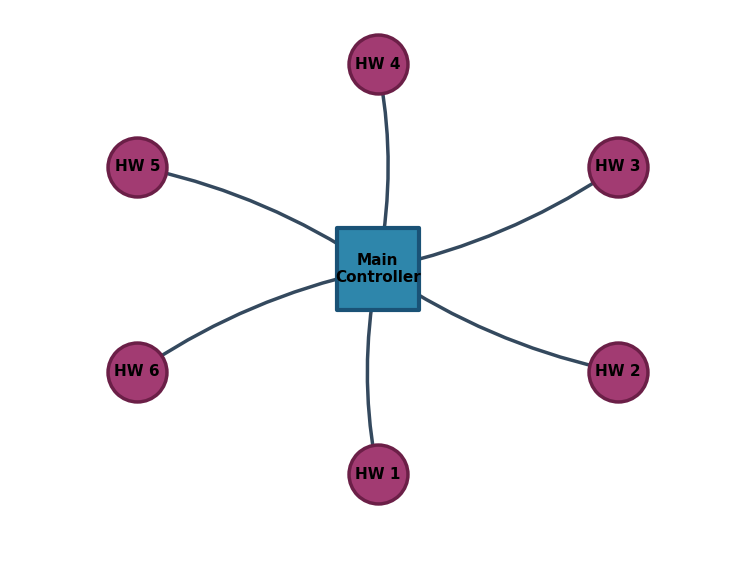
\includegraphics[width=0.95\linewidth]{obr/Star_topology.png}
    \caption{Centralizovaná topológia}
    \label{fig:centralizovana}
\end{minipage}\hfill
\begin{minipage}{0.48\textwidth}
    \centering
    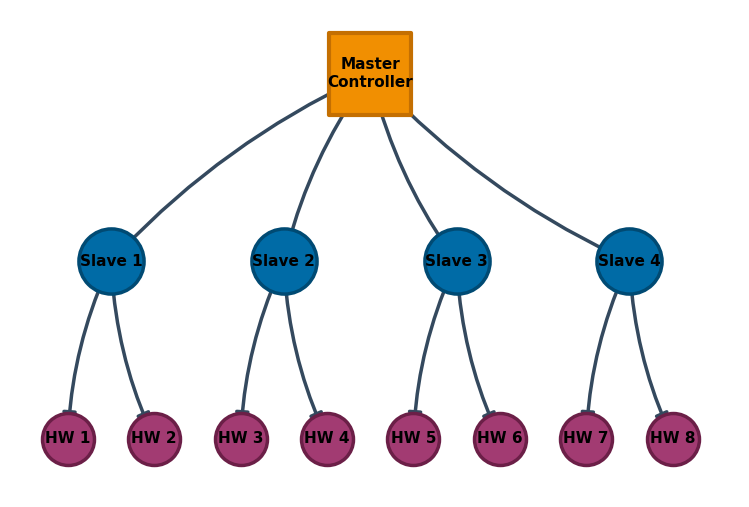
\includegraphics[width=0.95\linewidth]{obr/Pyramid_topology.png}
    \caption{Distribuovaná topológia}
    \label{fig:distribuovana}
\end{minipage}
\end{figure}

V~prostredí distribuovaných systémov sa čoraz viac presadzuje koncept \textit{Cyber-Physical Systems} (CPS), ktoré integrujú výpočtové a~fyzické komponenty do jedného celku. Tieto systémy umožňujú presnú synchronizáciu medzi digitálnym obsahom a~fyzickými efektmi, čo je nevyhnutné pre vytvorenie imerzívneho zážitku \cite{museum_immersive_design}. Výzvou pri návrhu takýchto systémov zostáva predpovedanie priepustnosti a~odozvy siete, čo si vyžaduje využitie formalizovaných metód, ako sú konečné stavové automaty (\textit{Finite State Machine}, FSM) \cite{distributed_control_modeling}.

% ------------------------------------------------------------------
\section{Existujúce prístupy k~riadeniu expozícií}
\label{existujuce-pristupy}

V~súčasnosti neexistuje jedno univerzálne riešenie pre implementáciu interaktívnych expozícií. Realizátori si spravidla vyberajú medzi viacerými kategóriami, z~ktorých každá má svoje špecifiká, výhody a~obmedzenia. Výber konkrétnej platformy závisí od požiadaviek na spoľahlivosť, synchronizáciu multimédií a~dostupný rozpočet.

\subsection{Priemyselné riadiace systémy (PLC)}
\label{plc-systemy}

V~oblasti klasickej automatizácie sú dlhoročným štandardom Programovateľné logické automaty (PLC) od výrobcov ako \textbf{Siemens, Beckhoff či Mitsubishi} \cite{plc_journal}. Ich hlavnou výhodou je determinizmus, teda zaručená odozva systému na vstup v~presne definovanom čase \cite{plc_journal}. Táto vlastnosť je kritická pre bezpečnostné funkcie, ale pre bežné interaktívne inštalácie v~múzeách je často nadbytočná.

PLC sú však primárne navrhnuté na prácu s~logickými signálmi a~narážajú na výrazné obmedzenia v~oblasti multimédií. Absencia natívnych HDMI portov a~neschopnosť priamo dekódovať video súbory vyžadujú použitie externých mediálnych prehrávačov \cite{rpi_esp32_scada}. Vysoká cena licencií a~hardvéru navyše robí tieto systémy neprístupnými pre menšie kultúrne inštitúcie \cite{interactive_small_museums}.

\subsection{Profesionálne show-control systémy}
\label{show-control}

Špecializované systémy ako \textbf{Medialon} a~\textbf{Alcorn McBride} sú navrhnuté priamo pre potreby tematických parkov a~múzeí \cite{medialon_sumble, alcornmcbride}. Na rozdiel od priemyselných PLC ich architektúra nie je postavená na cyklickom vykonávaní kódu, ale na princípe časovej osi (\textit{timeline}), čo umožňuje operátorovi precízne synchronizovať udalosti v~čase, podobne ako pri editácii videa \cite{alcornmcbride_history}.

Tieto systémy natívne integrujú protokoly používané v~zábavnom priemysle \cite{simpson_show}:
\begin{itemize}
    \item \textbf{SMPTE Timecode:} Pre presnú časovú synchronizáciu medzi zvukom, obrazom a~fyzickými efektmi.
    \item \textbf{DMX512 / Art-Net:} Pre komplexné riadenie scénického osvetlenia \cite{dmx_basics}.
    \item \textbf{OSC (Open Sound Control):} Pre sieťovú komunikáciu s~multimediálnymi servermi.
\end{itemize}

Napriek vysokej spoľahlivosti je ich hlavnou nevýhodou proprietárna povaha, ktorá vytvára závislosť na dodávateľovi a~znemožňuje flexibilné rozširovanie systému o~vlastné hardvérové riešenia bez drahých certifikácií \cite{showcontrol_comparison}.

\subsection{Otvorené IoT a~SBC systémy}
\label{otvorene-iot}

Treťou, čoraz populárnejšou kategóriou sú otvorené a~modulárne systémy postavené na princípoch Internetu vecí (IoT). Tento segment zaznamenal za posledné desaťročie prudký nárast vďaka dostupnosti jednodoskových počítačov (SBC) a~výkonných mikrokontrolérov \cite{microcontrollers_museum_arxiv}. Na rozdiel od uzavretých systémov táto kategória využíva open-source softvér a~štandardné programovacie jazyky (Python, C++), čo poskytuje vývojárom maximálnu slobodu pri tvorbe unikátnych interakcií \cite{computational_frameworks_art}.

Architektúra je typicky rozdelená na dve funkčné úrovne \cite{rpi_esp32_scada}:
\begin{itemize}
    \item \textbf{Výkonné centrálne jednotky (SBC):} Jednodoskové počítače s~plnohodnotným operačným systémom (najčastejšie na báze Linuxu) slúžiace na koordináciu celého systému a~predovšetkým na náročné multimediálne úlohy.
    \item \textbf{Distribuované periférie:} Koncové prvky (senzory, osvetlenie, mechanika) riadené samostatnými mikrokontrolérmi, ktoré fungujú ako inteligentné sieťové uzly schopné spracúvať dáta lokálne \cite{distributed_control_modeling}.
\end{itemize}

Využitie platforiem ako Raspberry Pi pre centrálnu logiku a~ESP32 pre distribuované uzly umožňuje budovanie systémov, ktoré kombinujú výpočtovú silu potrebnú pre multimédiá s~nízkoúrovňovým riadením hardvéru \cite{rpi_esp32_scada}. Tento prístup je nielen finančne efektívny, ale vďaka rozsiahlej komunite a~dostupnosti knižníc umožňuje rýchle prototypovanie aj veľmi komplexných nelineárnych scenárov \cite{interactive_small_museums}.

% ------------------------------------------------------------------
\section{Komunikačné protokoly}
\label{komunikacne-protokoly}

V~distribuovanom systéme je voľba komunikačného protokolu rozhodujúcim faktorom pre plynulosť interakcie \cite{rpi_esp32_scada}. Pri výbere sa zvažujú parametre ako latencia, réžia protokolu a~spoľahlivosť doručenia v~rámci lokálnej siete \cite{mqtt_http_latency}.

\subsection{Prenosové médiá: drôtové vs. bezdrôtové}
\label{prenosove-media}

Pri inštaláciách v~múzeách je kritickým faktorom spôsob prepojenia komponentov. Tradičné drôtové zbernice (RS-485, Ethernet) ponúkajú vysokú spoľahlivosť a~deterministickú komunikáciu. Ich nevýhodou je nutnosť fyzickej kabeláže ku každému prvku, čo môže byť v~historických priestoroch problematické \cite{rpi_esp32_scada}.

Bezdrôtové technológie (Wi-Fi, Bluetooth, Zigbee) eliminujú potrebu kabeláže a~výrazne zvyšujú flexibilitu systému \cite{rpi_esp32_scada}. Mikrokontroléry ESP32 majú vstavané Wi-Fi a~priamo sa pripájajú do lokálnej siete, čo umožňuje jednoducho premiestňovať interaktívne prvky bez nových prípojok \cite{esp32_comprehensive}.

\subsection{Aplikačné protokoly}
\label{aplikacne-protokoly}

Tradičný protokol \textbf{HTTP}, hoci je univerzálne podporovaný, sa pre interaktívne IoT systémy javí ako nevhodný \cite{rpi_esp32_scada}. Model request/response vyžaduje od koncového zariadenia neustále dopytovanie (polling) servera, čo vedie k~vysokej latencii a~zbytočnej záťaži procesora aj sieťového média \cite{mqtt_vs_http_hivemq}. Každá HTTP správa nesie objemné textové hlavičky, ktoré sú neefektívne pre prenos krátkych riadiacich príkazov \cite{mqtt_http_power}.

\textbf{WebSocket} predstavuje lepšiu alternatívu pre aplikácie vyžadujúce obojsmerný tok dát, pretože umožňuje udržiavať trvalé spojenie \cite{rpi_esp32_scada, mqtt_websocket_comparison}. Je obzvlášť vhodný pre webové riadiace panely (dashboards), avšak jeho implementácia na jednoduchých mikrokontroléroch je relatívne zložitá a~vyžaduje viac pamäťových zdrojov ako optimalizované IoT protokoly \cite{mqtt_websocket_comparison}.

\textbf{MQTT} (\textit{Message Queuing Telemetry Transport}), definovaný ako ISO štandard ISO/IEC 20922:2016, je v~súčasnosti najrozšírenejším protokolom pre distribuované IoT systémy \cite{mqtt_iso_standard}. Funguje na modeli \textit{Publish/Subscribe}, kde centrálny sprostredkovateľ (broker) distribuuje správy prihláseným klientom na základe hierarchických tém (topics) \cite{mqtt_m2m_survey}. Prenos správ prebieha nad trvalým TCP/IP spojením.

Experimentálne štúdie potvrdzujú, že MQTT v~lokálnom sieťovom prostredí výrazne prekonáva alternatívne protokoly z~hľadiska latencie a~stability \cite{mqtt_websocket_comparison}. Priemerná odozva $11{,}04\,\text{ms}$ pri použití MQTT QoS\,0 je $3{,}76$-násobne nižšia v~porovnaní s~protokolom WebSocket ($41{,}54\,\text{ms}$), čo je kľúčové pre synchrónne efekty, kde by akékoľvek zreteľné oneskorenie narušilo imerziu návštevníka \cite{mqtt_websocket_comparison}.

Protokol MQTT definuje tri úrovne kvality služieb (QoS), ktoré umožňujú prispôsobiť komunikáciu podľa požiadaviek \cite{mqtt_m2m_survey}:

\begin{table}[h]
\centering
\caption{Úrovne kvality služby (QoS) v~MQTT}
\label{tab:mqtt-qos}
\begin{tabular}{|c|l|p{7cm}|}
\hline
\textbf{QoS} & \textbf{Úroveň} & \textbf{Použitie} \\
\hline
0 & At most once & Menej kritické dáta (napr. pravidelné senzorické hodnoty), bez potvrdenia \\
\hline
1 & At least once & Dôležité správy, možné duplikáty, s~potvrdením \\
\hline
2 & Exactly once & Kritické povely (napr. pohyb motora), garantované doručenie presne raz \\
\hline
\end{tabular}
\end{table}

Okrem QoS poskytuje MQTT mechanizmus \textit{Last Will and Testament} (LWT), ktorý umožňuje brokeru automaticky informovať ostatné časti systému, ak dôjde k~neočakávanému odpojeniu zariadenia \cite{mqtt_lwt_review}. Tento mechanizmus je v~kombinácii so zostatkovými (\textit{retained}) správami kľúčový pre budovanie samoopravných systémov, ktoré dokážu po výpadku napájania okamžite obnoviť svoj stav \cite{mqtt_lwt_review, mqtt_m2m_survey}.

% ------------------------------------------------------------------
\section{Hardvérové platformy pre IoT}
\label{hardverove-platformy}

Realizácia riadiaceho systému vyžaduje výber hardvéru pre dve úrovne: centrálnu jednotku určenú na koordináciu systému a~multimediálne funkcie, a~koncové uzly obsluhujúce senzory, aktuátory a~periférie v~priestore expozície.

\subsection{Jednodoskové počítače (SBC)}
\label{sbc-platformy}

Jednodoskové počítače (SBC), reprezentované platformou \textbf{Raspberry Pi}, sú vhodným riešením pre rolu centrálneho koordinátora expozície. Raspberry Pi ponúka dostatočný výkon pre beh plnohodnotného operačného systému Linux, čo umožňuje využitie pokročilých programovacích jazykov ako Python a~správu komplexnej logiky \cite{rpi_esp32_scada}.

Pre potreby moderných expozícií je kľúčová podpora multimediálnych rozhraní. Modely Raspberry Pi 4 a~5 disponujú duálnym micro-HDMI výstupom s~podporou rozlíšenia 4K a~hardvérovou akceleráciou dekódovania videa (H.264, H.265), čo im dáva značnú výhodu oproti priemyselným PLC \cite{rpi4_datasheet}. Zariadenie zároveň poskytuje 40-pinový GPIO header, cez ktorý možno pripojiť rôzne senzory a~aktuátory priamo bez externých adaptérov \cite{rpi4_datasheet}.

\subsection{Mikrokontroléry pre koncové uzly}
\label{mikrokontrolery}

Historicky populárna platforma \textbf{Arduino Uno} (8-bitový čip ATmega328P) sa v~kontexte moderného IoT stáva limitujúcou \cite{esp32_vs_arduino_norvi}. S~taktom 16\,MHz a~2\,kB RAM nie je schopná efektívne spracovávať sieťový TCP/IP stack a~súčasne parsovať komplexné JSON správy, čo vedie k~nestabilite systému pri vyššej sieťovej záťaži \cite{rpi_esp32_scada}.

Nástup čipu \textbf{ESP32} od spoločnosti Espressif priniesol radikálnu zmenu. Tento 32-bitový systém-na-čipe (SoC) integruje Wi-Fi a~Bluetooth konektivitu priamo v~module, disponuje dvojjadrovým procesorom s~taktom až 240\,MHz a~520\,kB SRAM \cite{esp32_comprehensive}. Dvojjadrová architektúra ESP32 je pre interaktívne expozície kritickou výhodou: jedno jadro môže byť vyhradené výhradne pre sieťovú komunikáciu (správa MQTT spojenia, Wi-Fi stack), zatiaľ čo druhé jadro v~reálnom čase obsluhuje kritické hardvérové úlohy, ako je PWM riadenie motorov alebo čítanie senzorov. Táto separácia eliminuje nežiaduci jitter v~mechanických pohyboch, ktorý by inak vznikal pri spracovávaní sieťovej réžie \cite{esp32_vs_arduino_ntchip}.

Počet priamo ovládaných výstupov môže byť v~rozsiahlych inštaláciách nedostačujúci. Na rozšírenie výstupnej kapacity bez obsadenia všetkých GPIO pinov sa využívajú sériové I2C expandéry (napr. PCF8574), ktoré cez dvojvodičovú zbernicu sprístupňujú až 8 dodatočných výstupov z~jednej adresy \cite{esp32_comprehensive}.

% ------------------------------------------------------------------
\section{Výkonová elektronika a riadenie fyzických efektov}
\label{vykonova-elektronika}

Riadiaci systém musí byť schopný bezpečne a~efektívne ovládať výkonové prvky rôznych napäťových hladín — od jednosmerných motorov a~nízkonapäťových záťaží (typicky 12\,V~DC) až po zariadenia pracujúce na sieťovom napätí 230\,V~AC.

\subsection{Riadenie jednosmerných (DC) motorov}
\label{dc-motory}

Na zmenu smeru otáčania a~reguláciu rýchlosti DC motorov sa využívajú moduly H-mostíkov. Staršie integrované obvody ako L293D alebo L298N, založené na Darlingtonových tranzistoroch, vykazujú v~moderných aplikáciách značné nedostatky \cite{darlington_vs_mosfet}. Ich vysoký saturačný úbytok napätia (typicky cez 1{,}5\,V) spôsobuje, že sa pri väčších prúdoch výrazne zahrievajú, čo vyžaduje masívne chladenie a~znižuje celkovú účinnosť systému \cite{darlington_vs_mosfet}.

Moderné H-mostíky prešli na MOSFET tranzistory s~extrémne nízkym odporom v~zopnutom stave, čím sa minimalizujú tepelné straty a~umožňuje sa riadenie prúdov desiatok ampérov takmer bez zahrievania. Pre menšie prúdy sú vhodné kompaktné integrované riešenia ako DRV88xx alebo TB6612FNG, ktoré disponujú ochranou proti prehriatiu, prepätiu a~skratu \cite{mosfet_h_bridge}. Pre väčšie inštalačné motory s~vyššími prúdovými nárokmi sa využívajú vysokoprúdové moduly (napr. BTS7960) s~maximálnym trvalým prúdom rádovo desiatky ampérov, ktoré sú schopné zvládať kinetické rázy pri rozbehu \cite{mosfet_h_bridge}.

\subsection{Spínanie záťaží a~reléové spínače}
\label{spinanie-sietoveho-napatia}

Pre ovládanie svetelných efektov, dymostrojov alebo iných záťaží v~expozíciách je nevyhnutné oddeliť nízkonapäťovú riadiacu logiku od výkonových obvodov. Reálne inštalácie pritom kombinujú záťaže na rôznych napäťových hladinách -- bežne 230\,V~AC (sieťové spotrebiče) aj 12\,V~DC (LED pásy, malé aktuátory). Pri výbere spínacej technológie sa v~praxi porovnávajú dve základné kategórie: \textbf{polovodičové relé} (SSR -- \textit{Solid State Relay}) a~\textbf{elektromechanické relé} \cite{ssr_guide}.

SSR nevyužívajú pohyblivé kontakty, čím eliminujú mechanické opotrebovanie, kontaktný oblúk a~akustický hluk \cite{ssr_guide}. Z~hľadiska elektromagnetickej kompatibility (EMC) je pri SSR kľúčová technika spínania: \textit{zero-cross} SSR spína záťaž výhradne v~momente prechodu sínusoidy nulou, čím minimalizuje prúdové špičky (\textit{inrush current}) a~elektromagnetické rušenie, zatiaľ čo \textit{random turn-on} SSR spína okamžite a~je vhodnejší pre induktívne záťaže a~fázové riadenie výkonu \cite{zero_cross_ssr, ssr_zero_cross_transformers}. Hlavnou nevýhodou SSR je obmedzená kompatibilita: väčšina bežne dostupných typov podporuje výhradne striedavé napätie (AC) a~vykazuje vyššiu citlivosť na prepätia \cite{ssr_guide}.

Elektromechanické relé spínajú fyzickým rozopnutím a~zopnutím kontaktov, vďaka čomu poskytujú úplnú galvanickú izoláciu a~sú schopné spínať záťaže rôzneho charakteru -- AC aj DC -- bez obmedzenia \cite{ssr_guide}. Nevýhodou sú pohyblivé časti s~obmedzenou životnosťou pri vysokej frekvencii spínania a~kontaktný oblúk pri induktívnych záťažiach. Vo forme kompletných priemyselných modulov s~optickým oddelením vstupov (optočleny) predstavujú elektromechanické relé overené riešenie pre aplikácie s~rôznorodými záťažami, nízkou frekvenciou spínania a~požiadavkou na prevádzkovú spoľahlivosť \cite{ssr_guide}.

% ------------------------------------------------------------------
\section{Dátové formáty pre konfiguráciu a~prenos}
\label{datove-formaty}

Pre štruktúrovanie prenášaných dát a~ukladanie konfigurácie je nutné zvoliť vhodný formát. V~kontexte IoT a~webových technológií sa najčastejšie porovnávajú textové formáty XML, YAML a~JSON \cite{iot_data_formats_review}.

\textbf{XML} (\textit{eXtensible Markup Language}) je dlhoročným priemyselným štandardom pre výmenu dát. V~prostredí embedded systémov je však považované za zastarané kvôli extrémnej verbosite a~zložitosti parserov, ktoré neúmerne zaťažujú pamäť mikrokontroléra \cite{iot_data_formats_review}.

\textbf{YAML} (\textit{YAML Ain't Markup Language}) si získal obľubu v~oblasti DevOps vďaka podpore komentárov a~maximálnej čitateľnosti pre človeka \cite{yaml_vs_json}. Avšak YAML parsery pre C++ sú pamäťovo náročné a~často chybové pri spracovávaní neštandardných odsadení, čo z~neho robí rizikovú voľbu pre real-time komunikáciu na mikrokontroléroch \cite{json_xml}.

\textbf{JSON} (\textit{JavaScript Object Notation}) sa stal de facto štandardom pre IoT vďaka optimálnej rovnováhe medzi čitateľnosťou a~strojospracovateľnosťou \cite{iot_data_formats_review}. JSON parsery, ako napríklad vysoko optimalizovaná knižnica ArduinoJson, umožňujú efektívnu prácu s~dátami aj na zariadeniach s~obmedzenou RAM \cite{arduinojson_reduce_memory}. Knižnica ArduinoJson vo verzii 7 prináša techniky ako filtrovanie vstupov a~zero-copy parsovanie, čím minimalizuje fragmentáciu heap pamäte pri parsovaní JSON správ \cite{arduinojson_v7}.

Okrem prenosu dát v~IoT komunikácii nachádza JSON uplatnenie aj ako \textbf{konfiguračný jazyk pre definíciu riadiacej logiky}. Vďaka svojej stromovej štruktúre umožňuje hierarchicky popisovať stavy, časové postupnosti akcií a~podmienky prechodov medzi nimi -- a~to v~podobe textového súboru editovateľného bez rekompilácie softvéru \cite{iot_data_formats_review}. Tento prístup oddeľuje obsah (scenár) od enginu (kód), čo je v~kontexte múzejných expozícií prakticky výhodné, keďže scenár môže upravovať aj netechnický personál \cite{yaml_vs_json}.

% ------------------------------------------------------------------
\section{Prístupy k~riadiacej logike expozície}
\label{riadiaca-logika}

Softvérová vrstva riadiaceho systému určuje, akým spôsobom sa definuje a~vykonáva scenár expozície. V~praxi sa stretávame predovšetkým s~dvoma prístupmi, ktoré sa líšia schopnosťou reagovať na externé udalosti.

Najjednoduchším riešením je \textbf{lineárny (sekvenčný) prístup}: scenár je pevná séria akcií vykonávaných v~pevnom poradí a~čase, bez možnosti vetvenia. Takéto systémy sú jednoduché na implementáciu a~postačujú pre pasívne inštalácie, kde sa obsah prehráva v~slučke bez závislosti od vstupu návštevníka \cite{computational_frameworks_art}. Ich zásadným obmedzením je, že vlákno čakajúce na uplynutie časovača nie je schopné súčasne reagovať na externé podnety, čo pri zložitejšom scenári vedie k~blokovaniu celého systému \cite{distributed_control_modeling}.

Pre interaktívne expozície, kde scenár musí reagovať na vstupy návštevníka (napr. stlačenie tlačidla, dohratý mediálny klip), je vhodnejší prístup založený na \textbf{konečnom stavovom automate} (\textit{Finite State Machine}, FSM). V~tomto modeli je správanie systému rozdelené do diskrétnych stavov; prechody medzi nimi sú podmienené konkrétnymi udalosťami (\textit{events}) -- uplynutím časovača, prijatím MQTT správy alebo dokončením prehrávania média \cite{distributed_control_modeling}. FSM umožňuje neblokujúce čakanie na viacero rôznych podmienok súčasne, čo je nevyhnutné pre dynamické vetvenie scenára \cite{computational_frameworks_art}.

% ------------------------------------------------------------------
\section{Zhrnutie rešerše}
\label{zhrnutie-reserse}

Analýza dostupných technických riešení preukázala, že pre špecifické potreby modulárnej, flexibilnej a~cenovo dostupnej muzeálnej inštalácie nie sú optimálne ani robustné priemyselné PLC (kvôli vysokej cene a~nutnosti centralizovanej kabeláže), ani uzavreté komerčné systémy show-control. Komplexná analýza dostupných technológií a~akademických zdrojov potvrdzuje, že pre potreby moderných interaktívnych expozícií je najvhodnejším prístupom vybudovanie distribuovaného IoT systému postaveného na otvorených hardvérových a~softvérových platformách \cite{computational_frameworks_art}. Tento model poskytuje flexibilitu potrebnú pre implementáciu komplexných, nelineárnych naratívov pri zachovaní nízkych nákladov a~vysokej udržateľnosti \cite{interactive_small_museums}.

Z~hľadiska komunikačnej vrstvy sa protokol MQTT ukázal ako jednoznačne vhodný pre distribuované systémy s~požiadavkou na nízku latenciu a~spoľahlivé doručovanie príkazov \cite{mqtt_websocket_comparison}. Centrálna riadiaca jednotka (SBC) pritom nesie zodpovednosť nielen za MQTT orchestráciu, ale aj za synchrónne prehrávanie audiovizuálneho obsahu v~reálnom čase \cite{rpi_esp32_scada, rpi4_datasheet}. Pre riadiacu logiku je pri interaktívnych expozíciách vhodný model konečného stavového automatu (FSM), ktorý umožňuje neblokujúce vetvenie scenára na základe externých udalostí \cite{distributed_control_modeling}. Konfigurácia takéhoto scenára vo formáte JSON poskytuje ľahko editovateľné a~strojovo spracovateľné definície stavov a~prechodov bez nutnosti zásahu do zdrojového kódu \cite{iot_data_formats_review}.